\documentclass[aspectratio=169]{beamer}
\usetheme{hogent}
\usecolortheme{hgwhite} % witte achtergrond, zwarte tekst

%% common.tex -- Code die in elk .tex-bestand terug komt

%% Packages

\usepackage[dutch]{babel}
\usepackage{graphicx}
\usepackage{comment,enumerate,hyperref}
\usepackage{amsmath,amsfonts,amssymb}
\usepackage{eurosym}
\usepackage{booktabs}
\usepackage{multicol,multirow}
\usepackage{listings}

\usepackage[outputdir=out]{minted}
%\usepackage{minted}

\usepackage[backend=biber,style=apa]{biblatex}
\DeclareLanguageMapping{dutch}{dutch-apa}

\usepackage{csquotes}

%% Variabelen, elk academiejaar aan te passen
\newcommand{\academicyear}{2023--2024 (revisie: \today)}
\newcommand{\lecturers}{Thomas Aelbrecht \and Thomas Parmentier \and Bert Van Vreckem}
\newcommand{\coursename}{Research Methods (IT)}

%% Macro's en commando's

%% \alertbox: een kader voor tekst die moet opvallen
\newcommand{\alertbox}[2][hgblue]{%
  \setbeamercolor{alertbox}{bg=#1,fg=white}
  \begin{beamercolorbox}[sep=2pt,center]{alertbox}
    \textbf{#2}
  \end{beamercolorbox}
}


%\addbibresource{rm1-werken-met-latex.bib}

%---------- Info over de presentatie ------------------------------------------

\title{Module 2. Working with \LaTeX.}
\subtitle{\coursename}
\author{\lecturers}   % Pas waarden aan in common.tex
\date{\academicyear}
\begin{document}

\begin{frame}
  \maketitle
\end{frame}

\begin{frame}
  \frametitle{Content}

  \tableofcontents
\end{frame}

\section{Introduction}

\subsection{Philosophy, history}

\begin{frame}
  \frametitle{Philosophy: why {\LaTeX}?}

  \begin{itemize}
    \item<+-> WYSIWYG text editors force authors to take care of the design.
    \item<+-> This results in bad, inconsistent design of documents.
    \item<+-> Good design of texts is a \textit{specialty}, and is best not left to the authors.
    \item<+-> {\LaTeX} ensures that authors need only think about \textit{content} and \textit{structure} of text.
  \end{itemize}
\end{frame}

\begin{frame}[plain]
  \frametitle{History}

  \begin{columns}[c]

    \column{.67\textwidth}
    \begin{itemize}
      \item<+-> 1977: Donald Knuth thinks the proofs of his book \textit{The art of Computer Programming} look horrible.
      \item<+-> 1978: he decided to write his own typesetting system, {\TeX}
      \item<+-> 1989: Version 3.0, since then only bugfix-releases (converging to \(\pi\))
      \item<+-> 1980s: Leslie Lamport develops markup language for {\TeX}: {\LaTeX}
    \end{itemize}

    \column{.33\textwidth}
    \begin{center}
      \only<1-3>{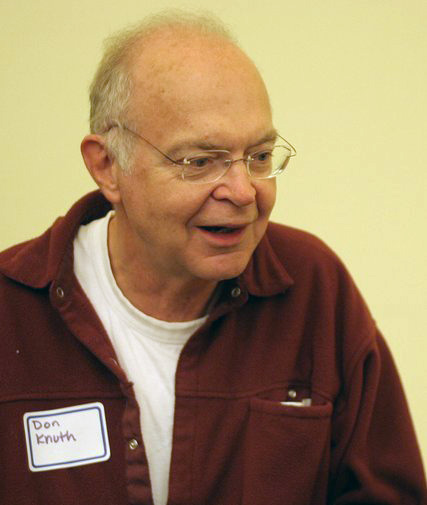
\includegraphics[width=\textwidth]{1/donald-knuth}}
      \only<4->{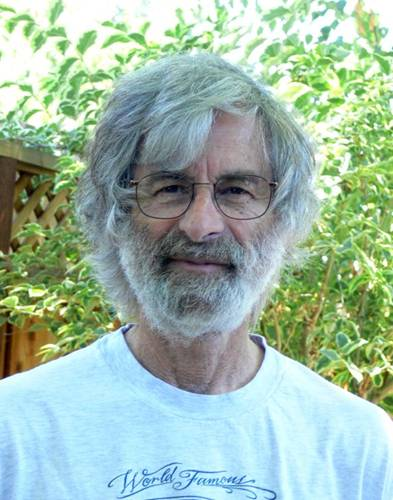
\includegraphics[width=\textwidth]{1/leslie-lamport}}
    \end{center}

  \end{columns}
\end{frame}

\subsection{Examples}

\begin{frame}
  \frametitle{Examples---papers}

  {\LaTeX} is the standard for scientific publications in computer sciences, maths, physics, etc..

  \begin{center}
    
\includegraphics[height=.6\textheight]{1/latex-paper}
  \end{center}

\end{frame}

\begin{frame}
  \frametitle{Examples---books}

  also: courses, theses, etc. 

  \begin{center}
    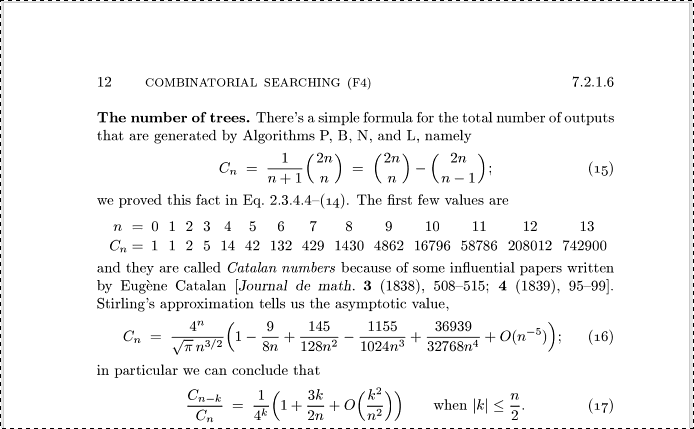
\includegraphics[height=.6\textheight]{1/latex-book}
  \end{center}

\end{frame}

\begin{frame}
  \frametitle{Examples---presentations}

  \begin{center}
    e.g. this presentation\ldots
  \end{center}

\end{frame}

\begin{frame}
  \frametitle{Advantages}

  \begin{itemize}
    \item<+-> Only take care of content, good and consistent design is guaranteed.
    \item<+-> Adapt style without adapting content.
    \item<+-> Text format \(\Rightarrow\) suitable for versioning system!
    \item<+-> Is the standard in different research domains, computer sciences among others
  \end{itemize}
\end{frame}


\begin{frame}
  \frametitle{Disadvantages}

  \begin{itemize}
    \item<+-> Steep learning curve \(\Rightarrow\) copy paste examples, use of information sources, getting help
    \item<+-> Sometimes the desired design is hard to accomplish (e.g. ~tables)
  \end{itemize}

  \uncover<1->{%
    \begin{center}
      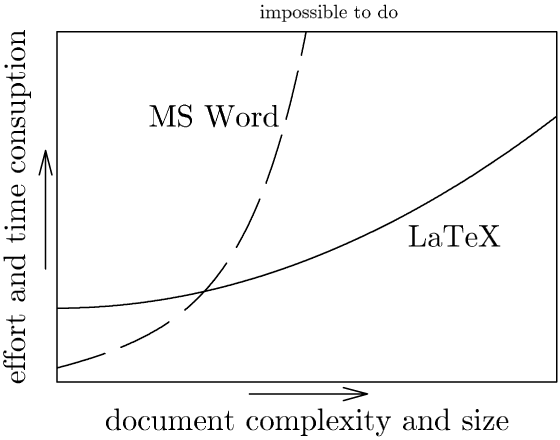
\includegraphics[height=.5\textheight]{1/word-vs-latex}
  \end{center}}
\end{frame}

\subsection{Getting help}

\begin{frame}
  \frametitle{Getting help}

  \begin{itemize}
    \item Tobias Oetiker, et al., \emph{The Not So Short Introduction to {\LaTeXe}}, 2011 (a.k.a. ``lshort'', versie 5.01)
    \item {\TeX} --- {\LaTeX} StackExchange (Q \& A site): \url{http://tex.stackexchange.com/}
    \item \emph{{\LaTeX} Wikibook}, \url{http://en.wikibooks.org/wiki/LaTeX}
    \item Manuals of packages (pdf)
  \end{itemize}

\end{frame}

\section{Getting started with {\LaTeX}}

\subsection{Document structure}

\begin{frame}
  \frametitle{Working method}

  \begin{itemize}
    \item<+-> Write text in  {\LaTeX}
    = text file! (markup language like HTML)
    \item<+-> Compile (possibly multiple times)
    \item<+-> Inspect result in PDF
  \end{itemize}
\end{frame}

\begin{frame}[fragile]
  \frametitle{{\LaTeX} commands}

  \begin{block}{Basic syntax}
    \verb|\command name[optional,arguments]{arg1}{arg2}|
  \end{block}

  \pause

  e.g. :

  \begin{itemize}
    \item<+-> \verb|\documentclass[a4paper,pdftex,12pt]{article}|
    \item<+-> \verb|\'{e}l\`{e}ve| \(\Rightarrow\) \'el\`eve
    \item<+-> \verb|\begin{itemize}|\\
    \verb|\item list|\\
    \verb|\end{itemize}|
  \end{itemize}

\end{frame}

\begin{frame}[fragile]
  \frametitle{Build a document }

  \begin{center}
    \alert{%
      \only<1>{Define the nature of the document (here: article)}
      \only<2>{``body'' of the document}
      \only<3>{Document content}
      \only<4>{Define extra functionality }
      \only<5>{Title, author ``preamble''}
      \only<6>{Title insertion in document}
    }
  \end{center}

  \begin{semiverbatim}
    \uncover<1->{\alert<1>{\\documentclass[a4paper,12pt]\{article\}}}
    \uncover<4->{\alert<4>{\\usepackage[dutch]\{babel\}}}
    \uncover<5->{\alert<5>{\\title\{Minimal \{\\LaTeX\} document\}}}
    \uncover<5->{\alert<5>{\\author\{Bert \{Van Vreckem\}\}}}
    \uncover<5->{\alert<5>{\\date\{\\today\}}}
    \uncover<2->{\alert<2>{\\begin\{document\}}}
    \uncover<6->{\alert<6>{\\maketitle}}
    \uncover<3->{\alert<3>{Lorem ipsum dolor sit amet, consectetur adipiscing elit.}}
    \uncover<2->{\alert<2>{\\end\{document\}}}
  \end{semiverbatim}

\end{frame}

\begin{frame}
  \frametitle{Result}

  \begin{center}
    
\includegraphics[height=.6\textheight]{1/minimaal-document}
  \end{center}
\end{frame}

\begin{frame}[fragile]
  \frametitle{Document types}

  \begin{center}
    \begin{semiverbatim}
      \\documentclass[\alert<2>{OPTIONS}]\{\alert<1>{TYPE}\}
    \end{semiverbatim}
  \end{center}

  \only<1>{%
    \begin{center}
      \begin{tabular}{ll}
        \toprule
        TYPE & nature of document \\
        \midrule
        \texttt{article} & article, paper, short text \\
        \texttt{beamer} & presentation \\
        \texttt{book} & book \\
        \texttt{report} & (long) report, thesis, paper, \ldots \\
      \end{tabular}
    \end{center}
  }
  \only<2>{%
    \begin{center}
      \begin{tabular}{ll}
        \toprule
        OPTION & nature of document \\
        \midrule
        \texttt{12pt} & 12-point letters (instead of 10pt) \\
        \texttt{a4paper} & A4 (instead of Am. Letter) \\
        \texttt{twocolumn} & common for articles \\
        \texttt{twoside} & for double sided printing \\
      \end{tabular}
    \end{center}
  }
\end{frame}

\begin{frame}[fragile]
  \frametitle{Document structure}

  \begin{center}
    \begin{tabular}{ll}
      \verb?\part? & (no influence on chapter numbers) \\
      \verb?\chapter? & (only in \texttt{book}, \texttt{report}) \\
      \verb?\section? & \\
      \verb?\subsection? & \\
      \verb?\subsubsection? & (not in \texttt{book}, \texttt{report}) \\
      \verb?\paragraph? & \\
      \verb?\subparagraph? & \\
      &\\
      \verb?\appendix? & from here on a \verb?\chapter? generates an  appendix  \\
      \verb?\label{?\texttt{\ldots}\verb?}? & for references (with \verb|\ref{LABEL}|)
    \end{tabular}
  \end{center}
\end{frame}

\begin{frame}[fragile]
  \frametitle{Preamble---Useful packages}

  \begin{description}
    \item[\texttt{\textbackslash{}usepackage\{amsfonts\}}] AMS math packages: extra mathematical
    \item[\texttt{\textbackslash{}usepackage\{amsmath\}}] symbols (e.g.\ number sets
    \item[\texttt{\textbackslash{}usepackage\{amssymb\}}] \(\mathbb{N}, \mathbb{R}, \mathbb{Z}, \mathbb{Q}\), etc.)
    \pause
    \item[\texttt{\textbackslash{}usepackage[dutch]\{babel\}}] Language settings: word split, commands for special characters (``dutch'' for NL)
    \pause
    \item[\texttt{\textbackslash{}usepackage\{eurosym\}}] Euro-symbol (\euro)
    \pause
    \item[\texttt{\textbackslash{}usepackage\{fancyhdr\}}] Page formatting with header and footer
    \pause
    \item[\texttt{\textbackslash{}usepackage\{graphicx\}}] Insert figures
  \end{description}
\end{frame}

\begin{frame}[fragile]
  \frametitle{Preamble---Useful packages}

  \begin{description}
    \item[\texttt{\textbackslash{}usepackage[pdftex,bookmarks=true]\{hyperref\}}] PDF gets clickable links \& references, table of contents \pause
    \item[\texttt{\textbackslash{}usepackage[utf8]\{inputenc\}}] use accents in text (e.g. é instead of \verb|\'e|) \pause
    \item[\texttt{\textbackslash{}usepackage\{listings\}}] Format source code \pause
    \item[\texttt{\textbackslash{}usepackage\{multirow\}}] Text in different cells in tables \pause
    \item[\texttt{\textbackslash{}usepackage\{rotating\}}] Tables and figures rotate \pause
    \item[\texttt{\textbackslash{}usepackage\{lipsum\}}] Filling text (lorem ipsum dolor sit amet\ldots)
  \end{description}
\end{frame}

\subsection{Text writing}

\begin{frame}[fragile]
 \frametitle{Tekst format}

 \begin{itemize}
   \item<+-> Special symbols ({\LaTeX} syntax): \% \$ \& \{ \} \textbackslash{} etc.: \\
   \begin{semiverbatim}
     \\\% \\\$ \\\& \\\{ \\\} \\textbackslash\{\}
   \end{semiverbatim}
   \item<+-> Ligatures: \textrm{fi fl ffi ffl} (automatic formatting)
   \item<+-> Accents: \'{e} \`{e} \^{e} \"{e} \={e} \c{c} etc.
   \begin{semiverbatim}
     \\'\{e\} \\`\{e\} \\^\{e\} \\"\{e\} \\=\{e\} \\c\{c\} etc.
   \end{semiverbatim}
   \item<+-> Ellipsis (\ldots): \texttt{\textbackslash{}ldots}
   \item<+-> Quotes: `single' ``double''
   \begin{verbatim}
   `single' ``double''
   \end{verbatim}
 \end{itemize}
\end{frame}

\begin{frame}[fragile]
 \frametitle{Letter styles}

 \begin{center}
   \begin{tabular}{ll}
     \toprule
     Command & result \\
     \midrule
     \verb?\emph{xxx}?   & \emph{Emphasis} (\textrm{\emph{italic}} of \textsf{\emph{`slanted'}})\\
     \verb?\textit{xxx}? & \textit{Italic text} \\
     \verb?\textbf{xxx}? & \textbf{Bold text} \\
     \verb?\texttt{xxx}? & \texttt{Mono spaced letters} \\
     \verb?\textrm{xxx}? & \textrm{Serif letters}  \\
     \verb?\textsf{xxx}? & \textsf{Sans Serif letters}  \\
     \verb?\textsc{xxx}? & \textsc{Small Caps} \\
   \end{tabular}
 \end{center}

\end{frame}

\begin{frame}[fragile]
 \frametitle{List environments}

 \begin{columns}[c]
   \column{.49\textwidth}
   \begin{verbatim}
   \begin{itemize}
   \item A part
   \item Another part
   \end{itemize}
   \end{verbatim}

   \column{.49\textwidth}
   \begin{itemize}
     \item A part
     \item Another part
   \end{itemize}
 \end{columns}

 \pause

 \begin{columns}[c]
   \column{.49\textwidth}
   \begin{verbatim}
   \begin{enumerate}
   \item A part
     \begin{enumerate}
     \item extra level
     \end{enumerate}
   \item Another part
   \end{enumerate}
   \end{verbatim}

   \column{.49\textwidth}
   \begin{enumerate}
     \item a part
     \begin{enumerate}
       \item extra level
     \end{enumerate}
     \item Another part
   \end{enumerate}
 \end{columns}

\end{frame}

\section{Figures, tables, etc.\ insert}

\subsection{Figures}

\begin{frame}[fragile,plain]
 \frametitle{Insert figures}

 \begin{columns}[c]
   \column{.65\textwidth}

\begin{semiverbatim}
\alert<1>{\\begin\{figure\}}
\alert<2>{\\includegraphics[width=\\textwidth]
 \{1/donald-knuth\}}
\alert<3>{\\caption\{\alert<4>{\\label\{fig:don\}}Donald Knuth, author of
 \{\\TeX\}\}}
\alert<1>{\\end\{figure\}}
\end{semiverbatim}

   \column{.35\textwidth}
   \begin{figure}
     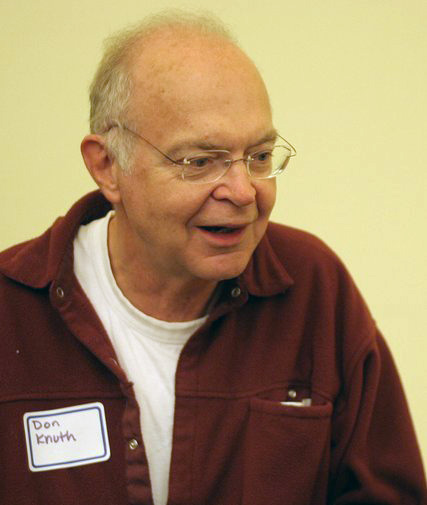
\includegraphics[width=\textwidth]{1/donald-knuth}
     \caption{\label{fig:don}Donald Knuth, author of {\TeX}}
   \end{figure}

 \end{columns}

\end{frame}

\subsection{Tabellen}

\begin{frame}[fragile]
 \frametitle{Insert tables}

 \begin{columns}[c]
   \column{.6\textwidth}
   \small
\begin{semiverbatim}
\alert<1>{\\begin\{table\}}
\alert<3>{\\begin\{tabular\}\{\alert<4>{l||c|r}\}}
\alert<4>{\\hline}
cel11 \alert<5>{&}
\alert<7>{\\multicolumn\{2\}\{c\}\{cell12\}} \alert<6>{\\\\}
\alert<4>{\\hline \\hline}
cell21 \alert<5>{&} cell22 \alert<5>{&}
\alert<7>{\\multirow\{2\}\{*\}\{cell23\}} \alert<6>{\\\\}
cell31 \alert<5>{&} cell32 \alert<5>{&} \alert<6>{\\\\}
\alert<3>{\\end\{tabular\}}
\alert<2>{\\caption\{An example of what you can do with tables\}
 \\label\{tab:example_table\}}
\alert<1>{\\end\{table\}}
\end{semiverbatim}

   \column{.4\textwidth}
   \begin{table}
     \begin{tabular}{l||c|r}
       \hline
       cel11 & \multicolumn{2}{c}{cell12} \\
       \hline \hline
       cel21 & cel22 & \multirow{2}{*}{cell23} \\
       cel31 & cel32 & \\
     \end{tabular}
     \caption{An example of what you can do with tables}
     \label{tab:example_tabel}
   \end{table}

 \end{columns}
\end{frame}

\subsection{Source code}

\begin{frame}[fragile]
 \frametitle{Insert source code}
 \framesubtitle{Simplest form: \texttt{verbatim}}

\begin{semiverbatim}
\alert{\\begin\{verbatim\}}
public class MyApp \{
 public static void main(String args[]) \{
   System.out.println("Hello World");
 \}
\}
\alert{\\end\{verbatim\}}
\end{semiverbatim}

 \(\Rightarrow\)

\begin{verbatim}
public class MyApp {
 public static void main(String args[]) {
   System.out.println("Hello World");
 }
}
\end{verbatim}

\end{frame}

\begin{frame}[fragile]
 \frametitle{Insert source code}
 \framesubtitle{\texttt{listings} package}

\begin{semiverbatim}
\\lstset\{\%
language=java,  breaklines=true,  numbers=left,
frame=single, caption=\{Mijn eerste Java-programma.\},
label=code:helloworld\}

\alert{\\begin\{lstlisting\}}
public class MyApp \{
 public static void main(String args[]) \{
   System.out.println("Hello World");
 \}
\}
\alert{\\end\{lstlisting\}}
\end{semiverbatim}

\end{frame}

\begin{frame}[fragile]
  \frametitle{Insert source code}
  \framesubtitle{\texttt{listings} package}

  \lstset{%
    language=java,    breaklines=true,
    numbers=left,     frame=single,
    caption={Mijn eerste Java-programma.},
    label=code:helloworld,
    gobble=2
  }

  \begin{lstlisting}
  public class MyApp {
    public static void main(String args[]) {
      System.out.println("Hello World");
    }
  }
  \end{lstlisting}

\end{frame}

\begin{frame}[fragile]
  \frametitle{Insert source code}
  \framesubtitle{\texttt{minted} package}

  \begin{semiverbatim}
  \\setminted\{%
    bgcolor=gray!20,gobble=2, linenos,
    numbers=left,frame=single\}

  \\begin\{minted\}\{java\}
    public class MyApp \{
      public static void main(String args[]) \{
        System.out.println("Hello World");
      \}
    \}
  \\end\{minted\}
  \end{semiverbatim}
\end{frame}


\begin{frame}[fragile]
  \frametitle{Insert source code}
  \framesubtitle{\texttt{minted} package}
  \setminted{bgcolor=gray!20,gobble=4,linenos,numbers=left,frame=single}
  \begin{minted}{java}
    public class MyApp {
      public static void main(String args[]) {
        System.out.println("Hello World");
      }
    }
  \end{minted}
\end{frame}

\subsection{Literature}

\begin{frame}[fragile]
  \frametitle{Literature}

  \begin{itemize}
    \item<+-> A literature list is an important part of a thesis
    \item<+-> Stringent rules for formatting (HOGENT: APA-stijl)
    \item<+-> {\LaTeX}, more precisely Bib{\LaTeX} helps:
    \begin{itemize}
      \item<+-> ``bibliografic database'' (in text format)
      \item<+-> Automatic correct formatting
      \item<+-> References from the text (\verb|\textcite{}|)
      \item<+-> Support via external tools (e.g. JabRef, Mendeley Desktop)
    \end{itemize}
  \end{itemize}

  \pause More later in this course!
\end{frame}

\section{Finally}

\begin{frame}[fragile]
 \frametitle{Finally}

  Many things haven't been discussed!

  \begin{itemize}
    \item<+-> Mathematical formulas, e.g.
    \begin{semiverbatim}
      \$x=-\\frac\{b \\pm \\sqrt\{b\^{}2 - 4ac\}\}\{2a\}\$
    \end{semiverbatim}
    \(x=-\frac{b \pm \sqrt{b^2 - 4ac}}{2a}\)
    \item<+-> Hundreds of packages (RTFM, Google is your friend)
    \item<+-> Presentations using Beamer (use e.g. \ the template at \url{https://github.com/HoGentTIN/presentatie-latex-sjabloon})

  \end{itemize}
\end{frame}

\end{document}
